\documentclass[12pt,twoside]{article}

\newcommand{\reporttitle}{Markowitz Model \& Rolling Window Back-Testing}
\newcommand{\reportauthor}{Rakesh Bali}
\newcommand{\reporttype}{Computational Finance with C++}
\newcommand{\cid}{01502703}

% include files that load packages and define macros
\input{includes} % various packages needed for maths etc.
\input{notation} % short-hand notation and macros

\usepackage{hyperref}
\usepackage{enumitem}
\usepackage{tikz}
\usetikzlibrary{arrows.meta, positioning, shapes.geometric}

%%%%%%%%%%%%%%%%%%%%%%%%%%%%

\begin{document}
% front page
\input{titlepage}

%%%%%%%%%%%%%%%%%%%%%%%%%%%% Main document


\section{Software Structure}

\textbf{Git Repository Link}\\
\text{\href{https://github.com/rakeshbali31/ComputationalFinanceCoursework}{https://github.com/rakeshbali31/ComputationalFinanceCoursework}}

\subsection{Classes Description}
\subsubsection{CsvReader}
\textbf{Purpose:} Reads CSV files and stores the data in a matrix.\\
\textbf{Key Methods:}
\begin{itemize}[nosep]
    \item \texttt{readCsv(const std::string\& filename, Matrix\& matrix)}: Reads a CSV file and stores the data in a matrix.
\end{itemize}

\subsubsection{Algorithm}
\textbf{Purpose:} Contains algorithms for mathematical computations, like the conjugate gradient method.\\
\textbf{Key Methods:}
\begin{itemize}[nosep]
    \item \texttt{conjugateGradient(const Matrix\& Q, const Vector\& b, const Vector\& x0, double tolerance)}: Solves a linear system using the conjugate gradient method.
\end{itemize}

\subsubsection{AssetCharacteristics}
\textbf{Purpose:} Provides methods to calculate statistical characteristics of assets.\\
\textbf{Key Methods:}
\begin{itemize}[nosep]
    \item \texttt{calculateMeans(const Matrix\& assetReturns, int startRow, int endRow)}: Calculates the mean returns of assets.
    \item \texttt{calculateCovariance(const Matrix\& assetReturns, const Vector\& means, int startRow, int endRow)}: Calculates the covariance matrix of asset returns.
\end{itemize}

\subsubsection{PortfolioSolver}
\textbf{Purpose:} Solves for the optimal portfolio weights given the asset returns and target return.\\
\textbf{Key Methods:}
\begin{itemize}[nosep]
    \item \texttt{solver() const}: Computes the optimal portfolio weights.
    \item \texttt{setAssetReturns(const Matrix\& matrix)}: Sets the asset returns.
    \item \texttt{setTargetReturn(double target)}: Sets the target return.
    \item \texttt{setRange(int start, int end)}: Sets the range for in-sample data. This sets the range of rows of asset returns to use for the calculation.
    \item \texttt{getAssetReturns() const}: Gets the asset returns.
    \item \texttt{getTargetReturn() const}: Gets the target return.
    \item \texttt{getRange() const}: Gets the in-sample data range.
\end{itemize}

\subsubsection{Backtest}
\textbf{Purpose:} Performs backtesting of the portfolio using out-of-sample data.\\
\textbf{Key Methods:}
\begin{itemize}[nosep]
    \item \texttt{backtest()}: Conducts the backtest and stores the results in out-of-sample-returns and out-of-sample-variances matrices.
    \item \texttt{getInputData()}: Gets input data for backtesting i.e., in-sample days and out-sample days.
    \item \texttt{displayResults() const}: Displays the backtest results.
    \item \texttt{saveResultsToCSV(const std::string\& filename) const}: Saves the backtest results to a CSV file.
\end{itemize}


\subsubsection{Matrix}
\textbf{Purpose:} Defines a matrix and provides basic linear algebra operations.\\
\textbf{Key Methods:}
\begin{itemize}[nosep]
    \item Operator overload for matrix and vector operations.
\end{itemize}

\subsection{Diagrams}
\subsubsection{Class Hierarchy}
\begin{tikzpicture}[
    class/.style={rectangle, draw=black, fill=gray!10, rounded corners, 
                  minimum height=2em, minimum width=10em, text centered, 
                  text width=10em},
    class box/.style={rectangle, draw=black, fill=white, rounded corners, 
                      minimum height=2em, minimum width=10em, text centered, 
                      text width=11em, font=\ttfamily},
    relation/.style={-{Stealth}, thin}
]

% Define classes
\node[class, below=of class1, yshift=-1cm] (class1) {PortfolioSolver};
\node[class, below=of class2, yshift=-4.5cm] (class2) {Backtest};

% Class contents
\node[class box, right=of class1] (class1Methods) {+ solver() \\ + setAssetReturns() \\ + setTargetReturn() \\ + setRange() \\ + getAssetReturns() \\ + getTargetReturn() \\ + getRange()};
\node[class box, right=of class2] (class2Methods) {+ backtest() \\ + getInputData() \\ + displayResults() \\ + saveResultsToCsv()};

% Relations
\draw[relation] (class1) -- (class2);

\end{tikzpicture}



\subsubsection{Relationships}
\begin{itemize}
    \item \textbf{CsvReader} is used by \textbf{Backtest} to read CSV files for input data.
    \item \textbf{Algorithm} provides mathematical methods used in \textbf{PortfolioSolver} for solving optimization problems.
    \item \textbf{AssetCharacteristics} provides methods to calculate asset statistics, which are used in \textbf{PortfolioSolver}.
    \item \textbf{PortfolioSolver} is the base class for \textbf{Backtest}, providing methods to solve for the optimal portfolio.
    \item \textbf{Backtest} extends \textbf{PortfolioSolver} to add functionality for backtesting the portfolio and also stores the backtesting results.
    \item The \textbf{Main} class is the entry point of the program. It initializes the \textbf{Backtest} object and coordinates the backtesting process.
\end{itemize}

\subsubsection{Class Diagram}
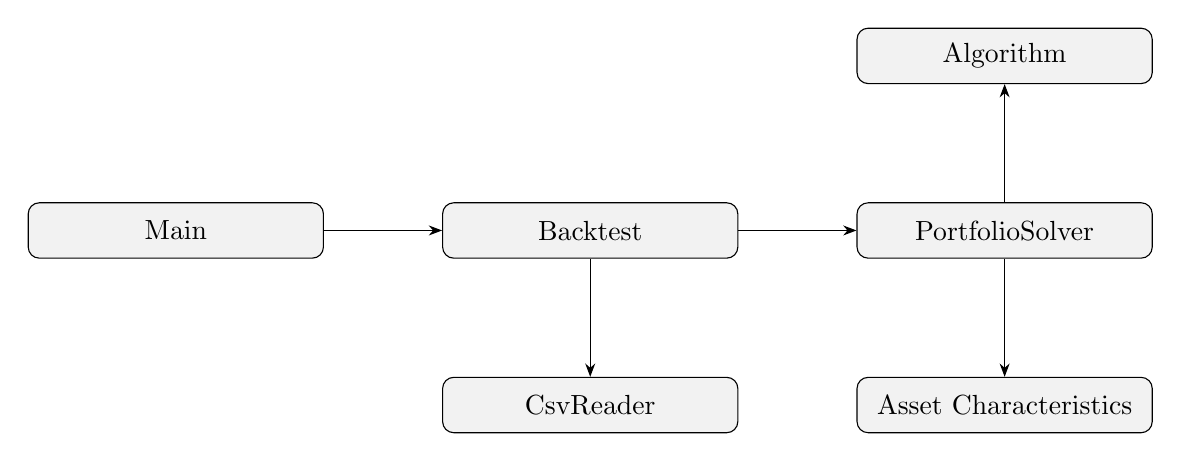
\begin{tikzpicture}[
    class/.style={rectangle, draw=black, fill=gray!10, rounded corners, 
                  minimum height=2em, minimum width=10em, text centered, 
                  text width=10em},
    relation/.style={-{Stealth}, thin}
]

% Define classes
\node[class] (class1) {Main};
\node[class, right=of class1, xshift=0.5cm] (class2) {Backtest};
\node[class, right=of class2, xshift=0.5cm] (class3) {PortfolioSolver};
\node[class, below=of class3, yshift=-0.5cm] (class4) {Asset Characteristics};
\node[class, above=of class3, yshift=0.5cm] (class5) {Algorithm};
\node[class, below=of class2, yshift=-0.5cm] (class6) {CsvReader};

% Relations
\draw[relation] (class1) -- (class2);
\draw[relation] (class2) -- (class3);
\draw[relation] (class3) -- (class4);
\draw[relation] (class3) -- (class5);
\draw[relation] (class2) -- (class6); 

\end{tikzpicture} 



\section{Evaluation}

\subsection{Plots}
Figure~\ref{fig:Stock_rets} illustrates the return charts for 83 FTSE 1000 companies. This plot confirms the accuracy of the data for all the stocks and ensures it is free from NaN values.\\

Figure~\ref{fig:OOS_rets} shows the average out-of-sample returns for different target returns over multiple rolling windows. Each line represents a target return, and the x-axis denotes the rolling window index. The average OOS returns fluctuate significantly over time. Higher target returns generally correspond to higher volatility in OOS returns. \\

Figure~\ref{fig:OOS_cum_rets}  presents the cumulative returns for each target return over the entire backtesting period. Each line represents the cumulative performance of a target return. Cumulative returns for higher target returns (e.g., 0.1) show significant growth compared to lower target returns. There are periods of drawdowns where cumulative returns decrease, particularly noticeable in mid-windows.\\

Figure~\ref{fig:Returns_vs_Risk} scatter plot compares the mean returns versus variance (risk) for different target returns during the first period. Colors indicate different target returns. There is a clear positive correlation between risk (variance) and return. Higher target returns correspond to higher variance, illustrating the risk-return trade-off. 


\begin{figure}[]
    \centering
    \includegraphics[width = 1.0\hsize]{./figures/stock_returns.png}
    \caption{Stock Returns Chart}
    \label{fig:Stock_rets}
\end{figure}


\begin{figure}[htbp!]
    \centering
    \includegraphics[width = 1.0\hsize]{./figures/mean_returns_plot.png} % span 1.0 times the horizontal size of the page
    \caption{Realised Rolling Window Average OOS Returns for each Target} 
    \label{fig:OOS_rets}
\end{figure}

\begin{figure}[]
    \centering
    \includegraphics[width = 1.0\hsize]{./figures/mean_cum_returns_plot.png}
    \caption{Cumulative Average OOS Returns for each target}
    \label{fig:OOS_cum_rets}
\end{figure}

\begin{figure}[]
    \centering
    \includegraphics[width = 1.0\hsize]{./figures/mean_returns_vs_variance.png}
    \caption{Risk vs Return plot for Period 1}
    \label{fig:Returns_vs_Risk}
\end{figure}


\subsection{Discussion}

The evaluation of the Markowitz model, as illustrated through these figures, underscores several key points:

\subsubsection{Efficient Frontier}
The plots collectively illustrate the efficient frontier, highlighting the trade-off between risk and return. Portfolios on the efficient frontier provide the best possible returns for a given level of risk.

\subsubsection{Optimal Portfolio}
The optimal portfolio for an investor depends on their risk tolerance. Higher risk tolerance would align with portfolios targeting higher returns (and accepting higher variance), while risk-averse investors would prefer portfolios with lower target returns and variance.

\subsubsection{Practical Application}
The rolling window analysis shows that the performance of the Markowitz model is dynamic and sensitive to changing market conditions. Regular rebalancing of the portfolio, as demonstrated, is essential to maintain optimal performance.

In conclusion, the Markowitz model provides a robust framework for portfolio optimization, balancing the trade-off between risk and return. The figures illustrate the practical outcomes of applying this model, showcasing its strengths and areas of variability across different market conditions.


\newpage
\section{Code}
\begin{itemize}
    \item Main.cpp
    \item Backtest.cpp
    \item PortfolioSolver.cpp
    \item AssetCharacteristics.cpp
    \item Algorithm.cpp
    \item CsvReader.cpp
    \item Matrix.cpp
\end{itemize}
\subsubsection{Main.cpp}
\scriptsize
\begin{verbatim}

#include <iostream>
#include "Backtest.h"

int main() {
    Backtest backtest;
    if(!backtest.getInputData()) {
        std::cout << "Exiting the program";
        return 0;
    }
    backtest.backtest();
    backtest.displayResults();
    backtest.saveResultsToCSV("results_python.csv");

}
\end{verbatim}
\subsubsection{Backtest.cpp}
\scriptsize
\begin{verbatim}

// Backtest.h

#ifndef BACKTEST_H
#define BACKTEST_H
#include <PortfolioSolver.h>

class Backtest: public PortfolioSolver {
private:
    int out_of_sample_period;
    Vector target_returns;
    Matrix out_of_sample_returns;
    Matrix out_of_sample_variance;

public:
    Backtest() : out_of_sample_period(10) {} // Default constructor initializing all members.
    Backtest(int out_of_sample_period, const Vector& target_returns) : out_of_sample_period(out_of_sample_period),
            target_returns(target_returns){}
    void backtest();
    int getInputData();
    void displayResults() const;
    void saveResultsToCSV(const std::string& filename) const;
};
#endif //BACKTEST_H

// Backtest.cpp

#include "Backtest.h"
#include <Algorithm.h>
#include <AssetCharacteristics.h>
#include <CsvReader.h>
#include <iomanip>
#include <iostream>
#include <fstream>


void Backtest::backtest() {
    const int num_of_days = getAssetReturns().size();
    const int in_sample_period = getEndRow() - getStartRow();

    for (const auto target_return:target_returns) {
        setRange(0, in_sample_period);
        int start = getStartRow(), end = getEndRow();
        Vector portfolioReturns;    // Local variable to store the portfolio returns for this target return
        Vector portfolioVariances;  // Local variable to store the portfolio variances for this target return
        setTargetReturn(target_return);
        while(end < num_of_days) {
            Vector weights = solver();

            Vector meanReturns = AssetCharacteristics::calculateMeans(getAssetReturns(), end, end+out_of_sample_period);
            double portfolioReturn = weights ^ meanReturns;
            portfolioReturns.push_back(portfolioReturn);

            Matrix covariance = AssetCharacteristics::calculateCovariance(getAssetReturns(), meanReturns, 
                                        end, end+out_of_sample_period);
            double portfolioVariance = weights ^ (covariance * weights);
            portfolioVariances.push_back(portfolioVariance);

            end += out_of_sample_period;
            start += out_of_sample_period;
            setRange(start, end);
        }
        out_of_sample_returns.push_back(portfolioReturns);
        out_of_sample_variance.push_back(portfolioVariances);
    }

}

int Backtest::getInputData() {
    std::string filename;
    int in_sample_period;

    //std::cout << "Enter the name of the excel file: "; std::cin >> filename;
    CsvReader reader;
    Matrix matrix;
    const bool success = reader.readCsv("asset_returns.csv", matrix);
    if (!success) {
        std::cerr << "Failed to read the CSV file." << std::endl;
        return 0;
    }

    //std::cout << "Enter the target return: "; std::cin >> targetReturn;
    double start=0.0, end=0.1, step=0.005;
    for (double value = start; value <= end; value += step) {
        target_returns.push_back(value);
    }

    std::cout << "Enter the insample period: "; std::cin >> in_sample_period;
    std::cout << "Enter the outsample period: "; std::cin >> out_of_sample_period;

    // Now set the values in PortfolioSolver
    setAssetReturns(matrix);
    setRange(0, in_sample_period);
    return 1;
}


void Backtest::displayResults() const {

    for (int i = 0; i < target_returns.size(); ++i) {
        std::cout << "Printing results for target return :: " << 
        std::fixed << std::setprecision(3) << target_returns[i] <<   std::endl << std::endl;

        Vector returns = out_of_sample_returns[i];
        Vector variances = out_of_sample_variance[i];
        const int array_size = returns.size();

        // Print header
        std::cout << std::setw(10) << "Period" << std::setw(20) << "Mean Return" << std::setw(20) << 
        "Variance" << std::endl;

        for (int j = 0; j < array_size; ++j) {
            // Print data for each period
            std::cout << std::setw(10) << j + 1 << std::setw(20) << std::fixed << std::setprecision(10) << 
            returns[j] << std::setw(20) << variances[j] << std::endl;
        }
        std::cout << std::endl;
    }
}


void Backtest::saveResultsToCSV(const std::string& filename) const {
    std::ofstream outFile(filename);

    for (int i = 0; i < target_returns.size(); ++i) {
        Vector returns = out_of_sample_returns[i];
        Vector variances = out_of_sample_variance[i];
        const int array_size = returns.size();

        // Write header to file
        outFile << "Period,Mean_Return,Variance,Target_Return\n";

        for (int j = 0; j < array_size; ++j) {
            // Write data for each period to file
            outFile << (j + 1) << "," << returns[j] << "," << variances[j] << "," << target_returns[i] << "\n";
        }
        outFile << "\n";
    }
    outFile.close();
}
\end{verbatim}


\subsubsection{PortfolioSolver.cpp}
\scriptsize
\begin{verbatim}

// PortfolioSolver.h

#ifndef PORTFOLIOSOLVER_H
#define PORTFOLIOSOLVER_H

#include <Matrix.h>

class PortfolioSolver {
private:
    Matrix assetReturns; // Stores returns of various assets within a specified range.
    double targetReturn; // Target return for the portfolio.
    int startRow;        // Starting index of the row in asset returns data.
    int endRow;          // Ending index of the row in asset returns data.

public:
    // Constructors
    PortfolioSolver() : targetReturn(0.0), startRow(0), endRow(0) {} // Default constructor initializing all members.
    explicit PortfolioSolver(const Matrix& matrix, double target, int start, int end)
        : assetReturns(matrix), targetReturn(target), startRow(start), endRow(end) {}
    // Constructor to initialize all properties.

    // Setters
    void setAssetReturns(const Matrix& matrix) { assetReturns = matrix; }
    void setTargetReturn(double target) { targetReturn = target; }
    void setRange(int start, int end) { startRow = start; endRow = end; }

    // Getters
    const Matrix& getAssetReturns() const { return assetReturns; }
    double getTargetReturn() const { return targetReturn; }
    int getStartRow() const { return startRow; }
    int getEndRow() const { return endRow; }

    // Solver
    Vector solver() const;
};

#endif // PORTFOLIOSOLVER_H


// PortfolioSolver.cpp

#include "PortfolioSolver.h"
#include <Algorithm.h>
#include <AssetCharacteristics.h>


Vector PortfolioSolver::solver() const {
    const int numAssets = assetReturns[0].size();
    const auto means = AssetCharacteristics::calculateMeans(assetReturns, startRow, endRow);
    const auto covariances = AssetCharacteristics::calculateCovariance(assetReturns, means, startRow, endRow);

    // Create the augmented matrices for optimization
    Matrix Q(numAssets + 2, Vector(numAssets + 2, 0.0));
    Vector b(numAssets + 2, 0.0);
    Vector x0(numAssets + 2, 1.0); // Initial guess

    // Fill Q and b based on the model
    for (int i = 0; i < numAssets; ++i) {
        for (int j = 0; j < numAssets; ++j) {
            Q[i][j] = covariances[i][j];
        }
        Q[i][numAssets] = -means[i];
        Q[i][numAssets + 1] = -1;

        Q[numAssets][i] = -means[i];
        Q[numAssets + 1][i] = -1;
    }
    b[numAssets] = -targetReturn;
    b[numAssets + 1] = -1;

    // Solve using the conjugate gradient method
    auto weights = Algorithm::conjugateGradient(Q, b, x0, 1e-6);
    weights.pop_back(); weights.pop_back(); // Removing lambda and M parameter
    return weights;
}


\end{verbatim}



\subsubsection{AssetCharacteristics.cpp}
\scriptsize
\begin{verbatim}

// AssetCharacteristics.h

#ifndef ASSET_CHARACTERISTICS_H
#define ASSET_CHARACTERISTICS_H

#include <Matrix.h>
#include <vector>

class AssetCharacteristics {
public:
    static Vector calculateMeans(const Matrix& returns, int startRow, int endRow);
    static Matrix calculateCovariance(const Matrix& returns, const Vector& means, int startRow, int endRow);
};

#endif // ASSET_CHARACTERISTICS_H

// AssetCharacteristics.cpp

#include "AssetCharacteristics.h"

using Vector = std::vector<double>;
using Matrix = std::vector<Vector>;

Vector AssetCharacteristics::calculateMeans(const Matrix& returns, int startRow, int endRow) {
    int numAssets = returns[0].size();
    Vector means(numAssets, 0.0);

    for (int i = 0; i < numAssets; ++i) {
        for (int k = startRow; k < endRow; ++k) {
            means[i] += returns[k][i];
        }
        means[i] /= (endRow - startRow);
    }
    return means;
}

Matrix AssetCharacteristics::calculateCovariance(const Matrix& returns, const Vector& means, int startRow, int endRow) {
    int numAssets = returns[0].size();
    Matrix covariance(numAssets, Vector(numAssets, 0.0));

    for (int i = 0; i < numAssets; ++i) {
        for (int j = i; j < numAssets; ++j) {  // Start from i to fill the upper triangle
            double sum = 0.0;
            for (int k = startRow; k < endRow; ++k) {
                double diff_i = returns[k][i] - means[i];
                double diff_j = returns[k][j] - means[j];
                sum += diff_i * diff_j;
            }
            covariance[i][j] = sum / (endRow - startRow - 1);  // Using N-1 (sample covariance)
            covariance[j][i] = covariance[i][j];  // Symmetric matrix
        }
    }

    return covariance;
}

\end{verbatim}


\subsubsection{Algorithm.cpp}
\scriptsize
\begin{verbatim}

//Algorithm.h

#ifndef ALGORITHM_H
#define ALGORITHM_H

#include "Matrix.h"

class Algorithm {
public:

    static Vector conjugateGradient(const Matrix& Q, const Vector& b, const Vector& x0, double tolerance);

};

#endif // ALGORITHM_H

//Algorithm.cpp

#include "Algorithm.h"


// Function to implement the conjugate gradient algorithm
Vector Algorithm::conjugateGradient(const Matrix& Q, const Vector& b, const Vector& x0, double tolerance) {
    Vector x = x0;
    Vector r = b - (Q * x); // Using operator- for subtraction
    Vector p = r;
    double rsold = r ^ r; // Using operator^ for dot product

    for (size_t i = 0; i < b.size(); ++i) {
        Vector Qp = Q * p;
        double alpha = rsold / (p ^ Qp); // Using operator^ for dot product
        x = x + (alpha * p); // Using operator+ for addition and operator* for scalar multiplication
        r = r - (alpha * Qp); // Using operator- for subtraction and operator* for scalar multiplication
        double rsnew = r ^ r; // Using operator^ for dot product

        if (sqrt(rsnew) < tolerance)
            break;

        double beta = rsnew / rsold;
        p = r + (beta * p); // Using operator+ for addition and operator* for scalar multiplication
        rsold = rsnew;
    }
    return x;
}

\end{verbatim}

\subsubsection{CsvReader.cpp}
\scriptsize
\begin{verbatim}

// CsvReader.h

#ifndef CSVREADER_H
#define CSVREADER_H

#include <Matrix.h>
#include <string>

class CsvReader {
public:
    static bool readCsv(const std::string& filename, Matrix& matrix);
};


#endif //CSVREADER_H


// CsvReader.cpp

#include "CsvReader.h"
#include <fstream>
#include <iostream>
#include <sstream>
#include <string>


bool CsvReader::readCsv(const std::string& filename, Matrix& matrix) {
    std::ifstream file(filename);
    if (!file.is_open()) {
        std::cerr << "Unable to open file: " << filename << std::endl;
        return false;
    }

    std::string line;
    while (getline(file, line)) {
        std::stringstream ss(line);
        std::string cell;
        Vector row;

        while (getline(ss, cell, ',')) {
            row.push_back(std::stod(cell));
        }
        matrix.push_back(row);
    }

    file.close();
    return true;
}
\end{verbatim}

\subsubsection{Matrix.cpp}
\scriptsize
\begin{verbatim}

// Matrix.h

#ifndef Matrix_h
#define Matrix_h

#include <vector>
using namespace std;

typedef vector<double> Vector;
typedef vector<Vector> Matrix;

Vector operator*(const Matrix& C,const Vector& V);
Vector operator*(const double& a,const Vector& V);
Vector operator+(const double& a,const Vector& V);
Vector operator+(const Vector& V,const Vector& W);
Vector operator-(const Vector& V, const double& a);
Vector operator-(const Vector& V,const Vector& W);
Vector operator*(const Vector& V,const Vector& W);
double operator^(const Vector& V,const Vector& W);

#endif


// Matrix.cpp

#include "Matrix.h"

// Multiplies a matrix by a vector
Vector operator*(const Matrix& C,const Vector& V)
{
   int d = C.size();
   Vector W(d);
   for (int j=0; j<d; j++)
   {
      W[j]=0.0;
      for (int l=0; l<d; l++) W[j]=W[j]+C[j][l]*V[l];
   }
   return W;
}

// Adds two vectors element-wise.
Vector operator+(const Vector& V,const Vector& W)
{
   int d = V.size();
   Vector U(d);
   for (int j=0; j<d; j++) U[j] = V[j] + W[j];
   return U;
}

// Adds a scalar to each element of a vector.
Vector operator+(const double& a,const Vector& V)
{
   int d = V.size();
   Vector U(d);
   for (int j=0; j<d; j++) U[j] = a + V[j];
   return U;
}

// Subtracts two vectors element-wise.
Vector operator-(const Vector& V,const Vector& W)
{
   int d = V.size();
   Vector U(d);
   for (int j=0; j<d; j++) U[j] = V[j] - W[j];
   return U;
}

// Subtracts a scalar to each element of a vector.
Vector operator-(const Vector& V, const double& a)
{
   int d = V.size();
   Vector U(d);
   for (int j=0; j<d; j++) U[j] = V[j] - a;
   return U;
}

// Multiplies each element of a vector by a scalar.
Vector operator*(const double& a,const Vector& V)
{
   int d = V.size();
   Vector U(d);
   for (int j=0; j<d; j++) U[j] = a*V[j];
   return U;
}

// Multiplies two vectors element-wise.
Vector operator*(const Vector& V,const Vector& W)
{
   int d = V.size();
   Vector U(d);
   for (int j=0; j<d; j++) U[j] = V[j] * W[j];
   return U;
}

// Computes the dot product of two vectors.
double operator^(const Vector& V,const Vector& W)
{
   double sum = 0.0;
   int d = V.size();
   for (int j=0; j<d; j++) sum = sum + V[j]*W[j];
   return sum;
}


\end{verbatim}


\end{document}


